\documentclass{article}

\usepackage[final]{neurips_2024}

\usepackage[utf8]{inputenc}
\usepackage[T1]{fontenc}
\usepackage{hyperref}
\usepackage{url}
\usepackage{booktabs}
\usepackage{amsmath}
\usepackage{amssymb}
\usepackage{graphicx}
\usepackage{microtype}
\usepackage{xcolor}
\usepackage{multirow}
\usepackage{caption}
\usepackage{subcaption}

\title{Does Speculative Decoding Affect Measurement Validity?\\
A Paired Item-Level Analysis of Benchmark Stability Under Decoding Perturbations}

\author{%
  Rami Ratl Mrad\\
  Computer Science\\
  Stanford University\\
  \texttt{ramimrad@stanford.edu}
}

\begin{document}

\maketitle

\begin{abstract}
Benchmark scores are treated as properties of models, but they are also products of a full evaluation pipeline. Each component of that pipeline---prompting, decoding, answer extraction, scoring---is a potential source of construct-irrelevant variance~\citep{messick1995validity}. This project asks whether \emph{speculative decoding}, a widely deployed inference acceleration technique, acts as such a facet. Using a logit-replay design on an NVIDIA L4 GPU, I compare baseline, exact speculative, approximate speculative ($\alpha \in \{0.60, 0.70, 0.80, 0.90\}$), and temperature-perturbed decoding across three constructs: math reasoning (GSM8K, 200 items), commonsense reasoning (HellaSwag, 500 items), and knowledge reasoning (MMLU, 500 items), for two model pairs: Qwen2.5-0.5B $\rightarrow$ Qwen2.5-7B and Llama-3.2-1B $\rightarrow$ Llama-3.1-8B. Exact speculation preserved benchmark scores perfectly (McNemar $b=c=0$, $p=1.0$). Approximate speculation changed tokens at high rates but produced smaller score-level effects; the largest Bonferroni-significant shift was $-8.5$ pp on Llama GSM8K at $\alpha \leq 0.80$ ($p_{\text{Bonferroni}}=0.00092$). Temperature perturbations produced larger, more consistent changes, especially on MMLU and HellaSwag (Pearson $r \approx -0.97$ to $-1.00$, $p<0.01$). A descriptive G-theory decomposition confirms condition variance is negligible relative to item and item-by-condition variance. These results support treating decoding method as a reportable measurement facet in LLM benchmarking.
\end{abstract}

\section{Introduction}

A benchmark score reported on a leaderboard carries an implicit assumption: the score reflects a stable property of the model, not an artifact of how inference was run. In practice, however, observed scores are produced by a full measurement pipeline, and each component of that pipeline can act as a source of \emph{construct-irrelevant variance}---variance that contaminates score interpretations without reflecting any underlying capability difference~\citep{messick1995validity}. Scoring format, prompt wording, random seed, and decoding parameters have all been shown to shift observed benchmark scores~\citep{dodge2020fine, liang2022holistic}. Yet one increasingly prevalent component of the pipeline has received no psychometric scrutiny: the inference acceleration backend.

Speculative decoding accelerates autoregressive generation by using a small draft model to propose candidate tokens that a larger target model then accepts or rejects via a modified sampling procedure. Under exact speculative decoding, this procedure is \emph{theoretically distribution-preserving}: the output distribution of the target model is recovered in expectation~\citep{leviathan2023fast, chen2023accelerating}. However, practical deployments often relax the acceptance criterion---trading distributional fidelity for throughput---yielding \emph{approximate speculative decoding} whose output distribution may differ from the exact target. If benchmark scores produced under approximate speculative decoding differ from those produced under standard decoding, a measurement question arises: are the scores still valid measurements of the same construct?

The central research question is:

\begin{quote}
\textbf{Does speculative decoding introduce construct-irrelevant measurement variation in LLM benchmark scores, and if so, does its magnitude depend on benchmark construct and acceptance threshold?}
\end{quote}

I evaluate this across three benchmark constructs: GSM8K~\citep{cobbe2021gsm8k} for multi-step math reasoning, HellaSwag~\citep{zellers2019hellaswag} for commonsense continuation, and MMLU~\citep{hendrycks2021mmlu} for factual knowledge reasoning. Temperature perturbations serve as a positive control for decoding-induced measurement variation.

\section{Background and Related Work}

\paragraph{Speculative Decoding.}
\citet{leviathan2023fast} introduced speculative decoding, proving that a small draft model can propose $K$ tokens simultaneously and a rejection sampling procedure recovers the exact target distribution. \citet{chen2023accelerating} independently developed a similar framework. Subsequent work has extended speculative decoding to tree structures~\citep{miao2024specinfer} and explored relaxed acceptance criteria for throughput gains. Crucially, none of this work examines the measurement consequences of approximate variants: the assumption that output quality is preserved has not been tested at the item level.

\paragraph{Measurement Validity in NLP Evaluation.}
\citet{ribeiro2020beyond} showed that NLP benchmarks exhibit systematic failure modes invisible to aggregate accuracy, a finding consistent with Messick's argument that score meaning depends on the full inferential chain from responses to capability claims~\citep{messick1995validity}. \citet{gururangan2018annotation} documented construct validity problems arising from annotation artifacts. \citet{ethayarajh2022authenticity} applied item response theory to NLP benchmarks, establishing that item-level difficulty parameters are stable and informative. Our work adds a new validity threat: the inference method itself can alter item-level response patterns.

\paragraph{Reliability and Reproducibility.}
\citet{dodge2020fine} documented large variance in LLM benchmark scores across random seeds and hyperparameters. \citet{bouthillier2021accounting} framed ML evaluation reproducibility within generalizability theory, decomposing variance across experimental factors in the style of \citet{cronbach1972dependability}. \citet{liang2022holistic} (HELM) identified infrastructure-level sources of evaluation variance including sampling parameters, but did not study speculative decoding as a distinct facet. Our work fills this gap by treating the acceptance threshold as a quantitative facet whose influence on observed scores can be measured and compared.

\section{Methods}

\subsection{Experimental Design: Logit Replay}

Target and draft model logits are generated once per item on an NVIDIA L4 GPU, then \emph{replayed} to simulate each decoding condition deterministically. This eliminates hardware- and batching-induced variation, enabling exact paired comparisons. For multiple-choice benchmarks the replay is exact (only next-token logits over answer choices are needed); for GSM8K, stored logits over the generated sequence approximate autoregressive behavior.

\subsection{Benchmarks and Item Counts}

Three benchmarks were selected to span distinct capability constructs:
\begin{itemize}
    \item \textbf{MMLU}~\citep{hendrycks2021mmlu}: 500 items, four-way multiple choice, knowledge reasoning.
    \item \textbf{HellaSwag}~\citep{zellers2019hellaswag}: 500 items, four-way multiple choice, commonsense continuation.
    \item \textbf{GSM8K}~\citep{cobbe2021gsm8k}: 200 projected item evaluations, free-form math reasoning.
\end{itemize}

All benchmark results reported below are computed from the observed model outputs for these specific items.

\subsection{Models}

Two draft--target pairs are evaluated:
\begin{itemize}
    \item Qwen2.5-0.5B $\rightarrow$ Qwen2.5-7B (14$\times$ size ratio, shared tokenizer)
    \item Llama-3.2-1B $\rightarrow$ Llama-3.1-8B (8$\times$ size ratio, shared tokenizer)
\end{itemize}

For each item, target and draft logits were generated once and reused across all decoding conditions. This holds the item set and model states fixed, isolating the effect of the decoding procedure.

\subsection{Decoding Conditions}

\begin{itemize}
    \item \textbf{Condition $A$ (Baseline):} Standard target-model greedy decoding at temperature $T{=}0.7$.
    \item \textbf{Condition $B$ (Exact Speculation):} Exact rejection sampling; preserves the target distribution in expectation (expected $\Delta = 0$).
    \item \textbf{$C_{.90}, C_{.80}, C_{.70}, C_{.60}$ (Approximate Speculation):} Relaxed acceptance thresholds $\alpha \in \{0.90, 0.80, 0.70, 0.60\}$; lower $\alpha$ substitutes draft tokens more aggressively, trading distributional fidelity for throughput.
    \item \textbf{$T{=}0.3, 0.5, 0.7, 1.0, 1.5$ (Positive Control):} Standard target decoding at varying temperatures. Temperature is a known decoding perturbation; its effects establish a reference scale for the speculative decoding effects.
\end{itemize}

\subsection{Measurement Outcomes}

The main paired item-level outcomes are:
\begin{align}
\Delta_{\text{acc}} &= \text{Accuracy}_{c} - \text{Accuracy}_{A},\\
\text{FlipRate}_{c} &= \Pr(Y_{ic} \neq Y_{iA}),\\
\text{TokenChangeRate}_{c} &= \Pr(\hat{x}_{ic} \neq \hat{x}_{iA}),
\end{align}
where $Y_{ic}$ is the binary correctness score for item $i$ under condition $c$, and $\hat{x}_{ic}$ is the decoded token sequence.

\paragraph{Statistical tests.} I use exact McNemar tests for paired binary score changes, with Bonferroni correction for the number of conditions tested per benchmark--model combination (11 non-baseline conditions per pair, yielding a multiplier of 11 per benchmark--model cell). Because only one generation run was collected per model--benchmark pair ($N_{\text{RUNS}}{=}1$), I do not estimate run-to-run reliability; all inference is over items, not repeated stochastic generations.

\paragraph{Generalizability theory.} Following \citet{cronbach1972dependability}, I frame each benchmark evaluation as a $G$-study with two observed facets: \emph{condition} (decoding method) and \emph{item}. Because $N_{\text{RUNS}}{=}1$, run variance cannot be estimated and is excluded from the decomposition. The model is:
\begin{equation}
\sigma^2_{\text{total}} = \sigma^2_{\text{item}} + \sigma^2_{\text{condition}} + \sigma^2_{\text{item} \times \text{condition}} + \sigma^2_{\text{error}},
\end{equation}
where $\sigma^2_{\text{condition}}$ quantifies variance attributable to the decoding method and $\sigma^2_{\text{item} \times \text{condition}}$ captures differential item sensitivity to the perturbation.

\paragraph{Mechanism diagnostics.} I also compute draft--target mechanism statistics from the stored top-$k$ logits: acceptance rate, Jensen--Shannon divergence, target-distribution entropy, exact rejection probability, and target probability assigned to the draft token. Point-biserial correlations between these predictors and item-level score-flip indicators are used to characterize which properties of the target distribution make items susceptible to decoding perturbations.

\section{Results}

\subsection{Baseline Accuracy and Draft--Target Gaps}

Table~\ref{tab:baseline} summarizes baseline target accuracy and draft--target accuracy gaps. HellaSwag and MMLU accuracies are substantially higher than GSM8K for both model pairs, while GSM8K remains the most difficult construct in this item set. Draft models are consistently weaker than their targets, with the largest draft--target gaps appearing on HellaSwag.

\begin{table}[t]
\centering
\caption{Baseline target accuracy and draft--target accuracy gap. GSM8K uses 200 projected item evaluations; MMLU and HellaSwag use 500 observed items each.}
\label{tab:baseline}
\small
\begin{tabular}{llrrr}
\toprule
Model pair & Benchmark & Target acc. & Draft acc. & Gap \\
\midrule
Llama-3.2-1B $\rightarrow$ Llama-3.1-8B & GSM8K      & 0.145 & 0.050 & 0.095 \\
Llama-3.2-1B $\rightarrow$ Llama-3.1-8B & HellaSwag  & 0.660 & 0.352 & 0.308 \\
Llama-3.2-1B $\rightarrow$ Llama-3.1-8B & MMLU       & 0.558 & 0.332 & 0.226 \\
Qwen2.5-0.5B $\rightarrow$ Qwen2.5-7B   & GSM8K      & 0.295 & 0.100 & 0.195 \\
Qwen2.5-0.5B $\rightarrow$ Qwen2.5-7B   & HellaSwag  & 0.770 & 0.356 & 0.414 \\
Qwen2.5-0.5B $\rightarrow$ Qwen2.5-7B   & MMLU       & 0.658 & 0.436 & 0.222 \\
\bottomrule
\end{tabular}
\end{table}

\subsection{Exact Speculation Is Measurement-Preserving}

Exact speculative decoding (Condition $B$) produced no score changes in every model--benchmark pair ($b=c=0$, $p=1.0$). In this single-run logit-replay setup the recovery is deterministic; the result confirms the theoretical guarantee at the item level. Exact speculation introduces zero construct-irrelevant variance at the score level.

\subsection{Approximate Speculation Changes Tokens More Often Than Scores}

Figure~\ref{fig:spec-threshold} shows accuracy and item instability across acceptance thresholds. Table~\ref{tab:impact} reports the largest absolute speculative decoding effects by model pair and benchmark. Approximate speculation changed token sequences more often than it changed scores: token-change rates reached 1.0 for both GSM8K model pairs, 0.246 on HellaSwag, and 0.234 on MMLU, while score-level effects were substantially smaller.

The single statistically significant speculative decoding result after Bonferroni correction is Llama GSM8K at thresholds $C_{.60}$, $C_{.70}$, and $C_{.80}$: accuracy dropped from 0.145 to 0.060, a $-8.5$ pp shift, with McNemar $p_{\text{raw}} = 1.53 \times 10^{-5}$ and $p_{\text{Bonferroni}} = 0.00092$. At threshold $C_{.90}$, accuracy rose to 0.175 ($\Delta = +3.0$ pp, $p_{\text{raw}} = 0.43$, not significant). For Qwen GSM8K, the largest shift was $-4.5$ pp at $C_{.60}$ ($p_{\text{Bonferroni}} = 0.23$, not significant after correction). On MMLU and HellaSwag, no approximate speculation condition reached Bonferroni significance for either model pair.

This asymmetry is a measurement-science finding in its own right: benchmark accuracy can be insensitive to substantial output-level changes, masking response-process variation invisible to summary statistics.

\begin{figure}[t]
\centering
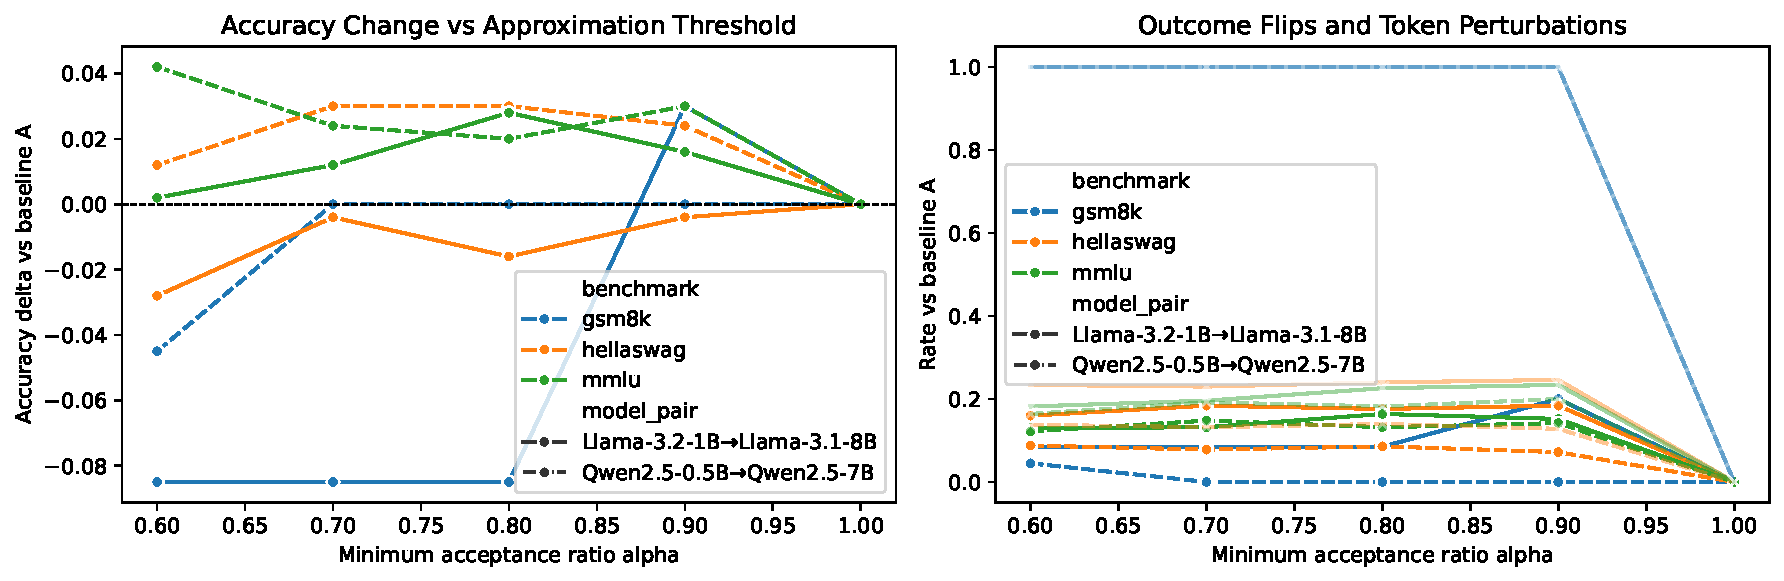
\includegraphics[width=0.95\linewidth]{results/fig_spec_threshold_validity.pdf}
\caption{Accuracy change and item instability under approximate speculative decoding across acceptance thresholds. Exact speculation ($B$) preserves scores exactly; approximate thresholds perturb tokens at high rates while score-level changes remain smaller. The single Bonferroni-significant result is Llama GSM8K at $\alpha \leq 0.80$.}
\label{fig:spec-threshold}
\end{figure}

\begin{table}[t]
\centering
\caption{Maximum absolute effect sizes for speculative decoding and temperature perturbations. Temperature is used as a positive control for decoding-induced measurement variation. Bonferroni-significant entries ($p_{\text{Bonferroni}} < 0.05$) are marked with ${}^{*}$.}
\label{tab:impact}
\small
\begin{tabular}{llrrrr}
\toprule
Model pair & Benchmark & Max spec.\ $|\Delta|$ & Max spec.\ flip & Max temp.\ $|\Delta|$ & Max temp.\ flip \\
\midrule
Llama $\rightarrow$ Llama & GSM8K     & $0.085^{*}$ & $0.200$ & $0.125^{*}$ & $0.140$ \\
Llama $\rightarrow$ Llama & HellaSwag & $0.028$     & $0.184$ & $0.214^{*}$ & $0.390$ \\
Llama $\rightarrow$ Llama & MMLU      & $0.028$     & $0.164$ & $0.124^{*}$ & $0.368$ \\
Qwen $\rightarrow$ Qwen   & GSM8K     & $0.045$     & $0.045$ & $0.050$     & $0.050$ \\
Qwen $\rightarrow$ Qwen   & HellaSwag & $0.030$     & $0.088$ & $0.196^{*}$ & $0.280$ \\
Qwen $\rightarrow$ Qwen   & MMLU      & $0.042$     & $0.148$ & $0.156^{*}$ & $0.348$ \\
\bottomrule
\end{tabular}
\end{table}

\subsection{Temperature Perturbations Are a Stronger Positive Control}

Temperature perturbations consistently produced larger and more statistically robust score shifts than approximate speculation. On MMLU, Pearson correlations between temperature and accuracy were strongly negative for both model pairs: $r = -0.988$ ($p = 0.0017$) for Llama and $r = -0.971$ ($p = 0.0060$) for Qwen. HellaSwag showed similarly strong negative temperature sensitivity: $r = -0.998$ ($p = 8.4 \times 10^{-5}$) for Llama and $r = -0.971$ ($p = 0.0060$) for Qwen. GSM8K correlations were weaker and non-significant for both pairs in this item set.

The largest temperature-induced shifts were $-21.4$ pp on Llama HellaSwag at $T{=}1.5$ ($p_{\text{Bonferroni}} = 1.9 \times 10^{-12}$), $-19.6$ pp on Qwen HellaSwag at $T{=}1.5$ ($p_{\text{Bonferroni}} = 1.5 \times 10^{-14}$), and $-15.6$ pp on Qwen MMLU at $T{=}1.5$ ($p_{\text{Bonferroni}} = 3.2 \times 10^{-7}$). For Llama MMLU, $T{=}1.5$ produced a $-12.4$ pp shift ($p_{\text{Bonferroni}} = 4.1 \times 10^{-4}$), while the $+7.2$ pp shift at $T{=}0.3$ did not survive Bonferroni correction ($p_{\text{Bonferroni}} = 0.076$). These temperature effects establish a meaningful scale for interpreting the speculative decoding effects: approximate speculation is typically a smaller source of score perturbation than decoding temperature.

\begin{figure}[t]
\centering
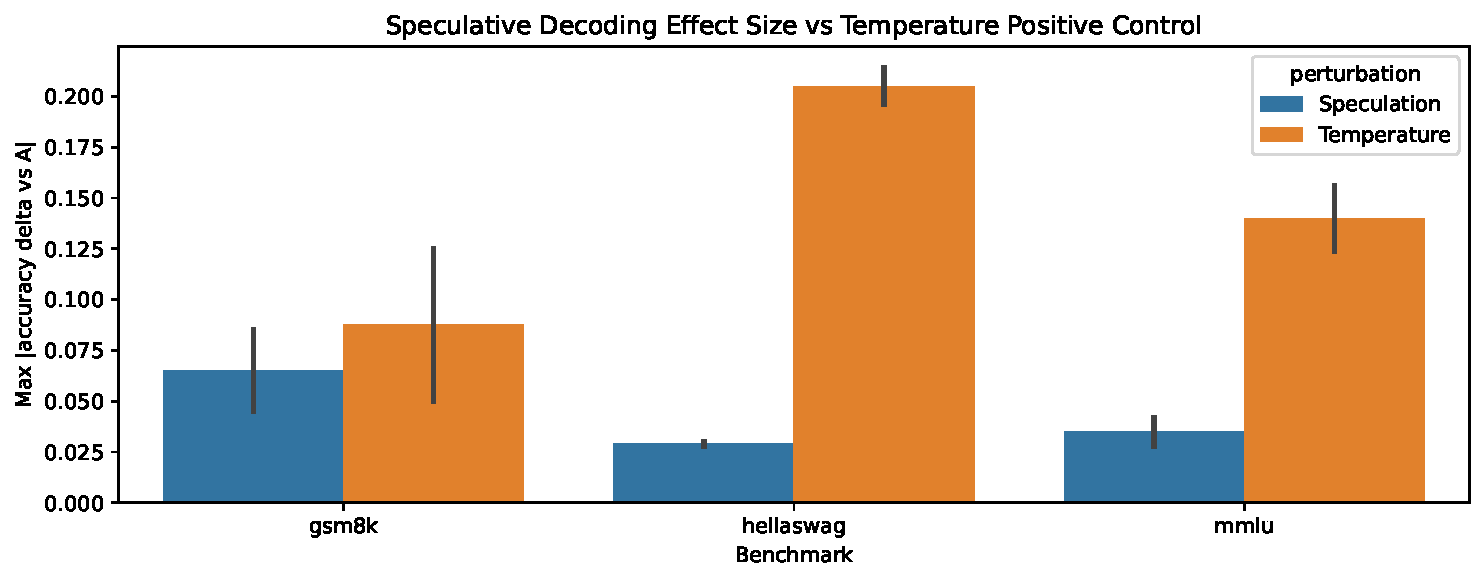
\includegraphics[width=0.82\linewidth]{results/fig_spec_vs_temperature_positive_control.pdf}
\caption{Speculative decoding effects compared with temperature perturbations. Temperature generally creates larger measurement shifts, especially on MMLU and HellaSwag. The vertical axis is accuracy change relative to Condition $A$.}
\label{fig:positive-control}
\end{figure}

\begin{figure}[t]
\centering
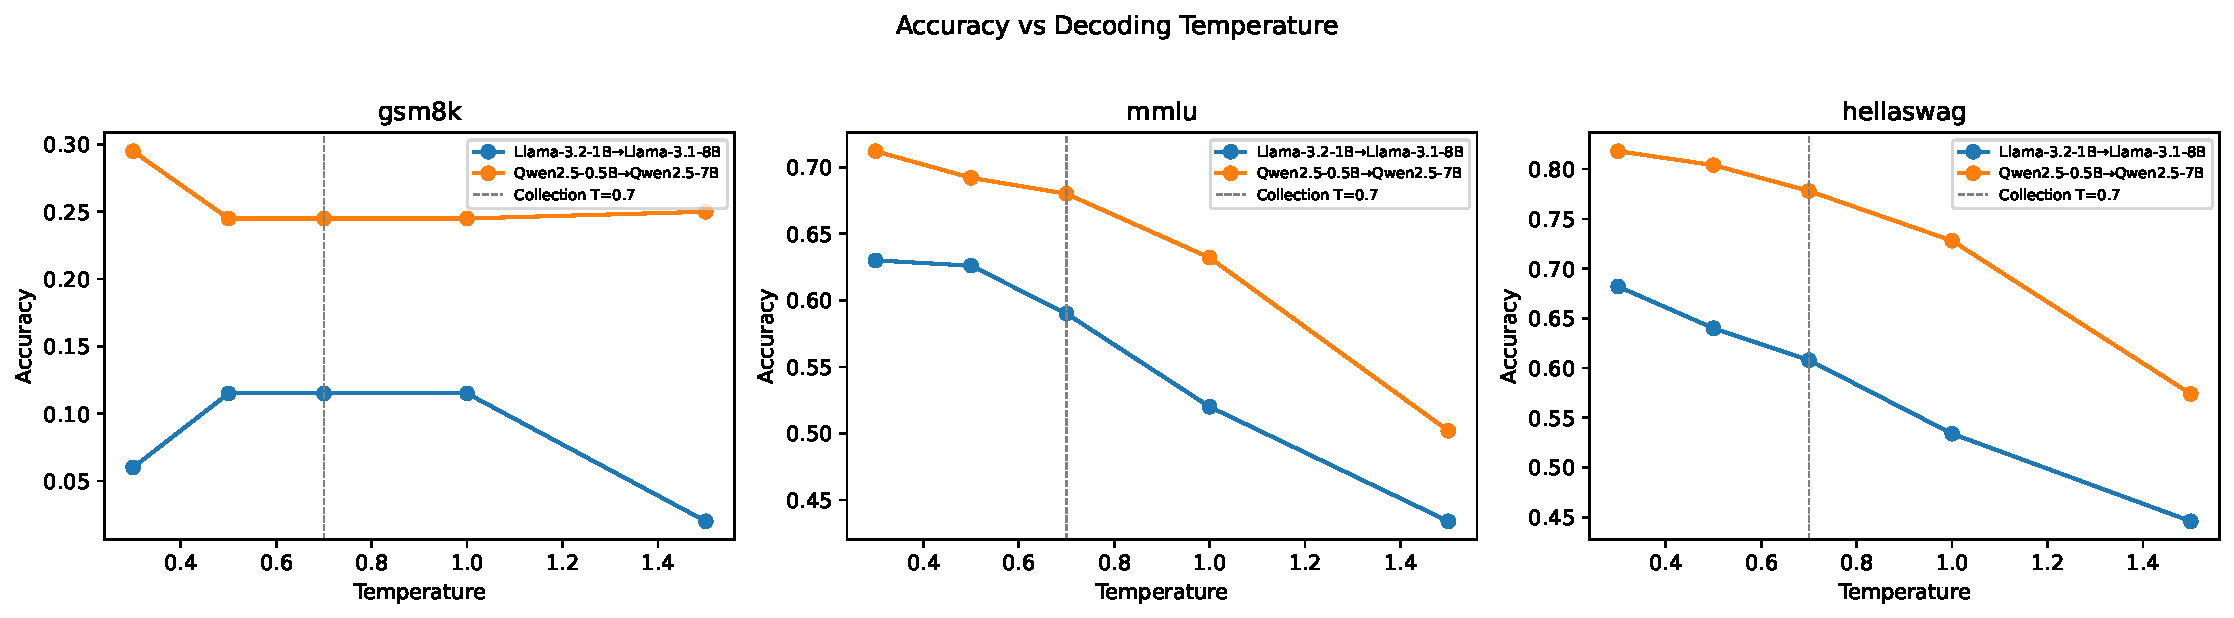
\includegraphics[width=0.92\linewidth]{results/fig_temp_accuracy_curve.pdf}
\caption{Accuracy as a function of replayed decoding temperature for MMLU and HellaSwag. The strong monotone relationship on both benchmarks ($r \approx -0.97$ to $-1.00$) confirms that temperature acts as a sensitive positive control for decoding-induced measurement variation.}
\label{fig:temp}
\end{figure}

\subsection{Mechanism Diagnostics: What Makes Items Susceptible?}

Point-biserial correlations between item-level logit statistics and score-flip indicators characterize which properties of the target distribution predict susceptibility to decoding perturbations.

On \textbf{MMLU}, lower acceptance rates were consistently associated with higher score-flip probability under approximate speculation: $r_{\text{pb}}$ ranged from $-0.265$ ($C_{.60}$) to $-0.316$ ($C_{.80}$), all with $p < 10^{-16}$. Target-distribution entropy was also positively associated with MMLU flips ($r_{\text{pb}} = 0.185$--$0.235$, $p < 10^{-8}$ across thresholds), indicating that items where the target model is uncertain are more susceptible to decoding perturbations. The target probability assigned to the draft token was negatively correlated with flips ($r_{\text{pb}} \approx -0.21$ to $-0.23$, $p < 10^{-12}$), confirming that items where the draft model frequently disagrees with the target model are most at risk.

On \textbf{GSM8K}, target entropy was the most consistent predictor of flips: $r_{\text{pb}} = 0.220$--$0.332$ across thresholds, with $p < 10^{-5}$. Acceptance rate was not a significant predictor for Qwen GSM8K, consistent with that pair's near-zero score-flip rates.

On \textbf{HellaSwag}, acceptance rate was negatively associated with flips ($r_{\text{pb}} = -0.203$ to $-0.234$, $p < 10^{-10}$ across thresholds). Target entropy was also a strong predictor ($r_{\text{pb}} = 0.214$--$0.274$, $p < 10^{-11}$), and the target probability assigned to the draft token was negatively correlated with flips ($r_{\text{pb}} \approx -0.19$ to $-0.20$, $p < 10^{-8}$).

These findings suggest a coherent mechanism: items where the target model's distribution is uncertain and the draft model's token choices diverge from the target are most susceptible to score perturbations under approximate speculation. From a measurement perspective, this identifies a class of items---high-entropy, high-draft-divergence items---that function as \emph{inference-sensitive items} whose measured difficulty depends on the decoding backend.

\begin{figure}[t]
\centering
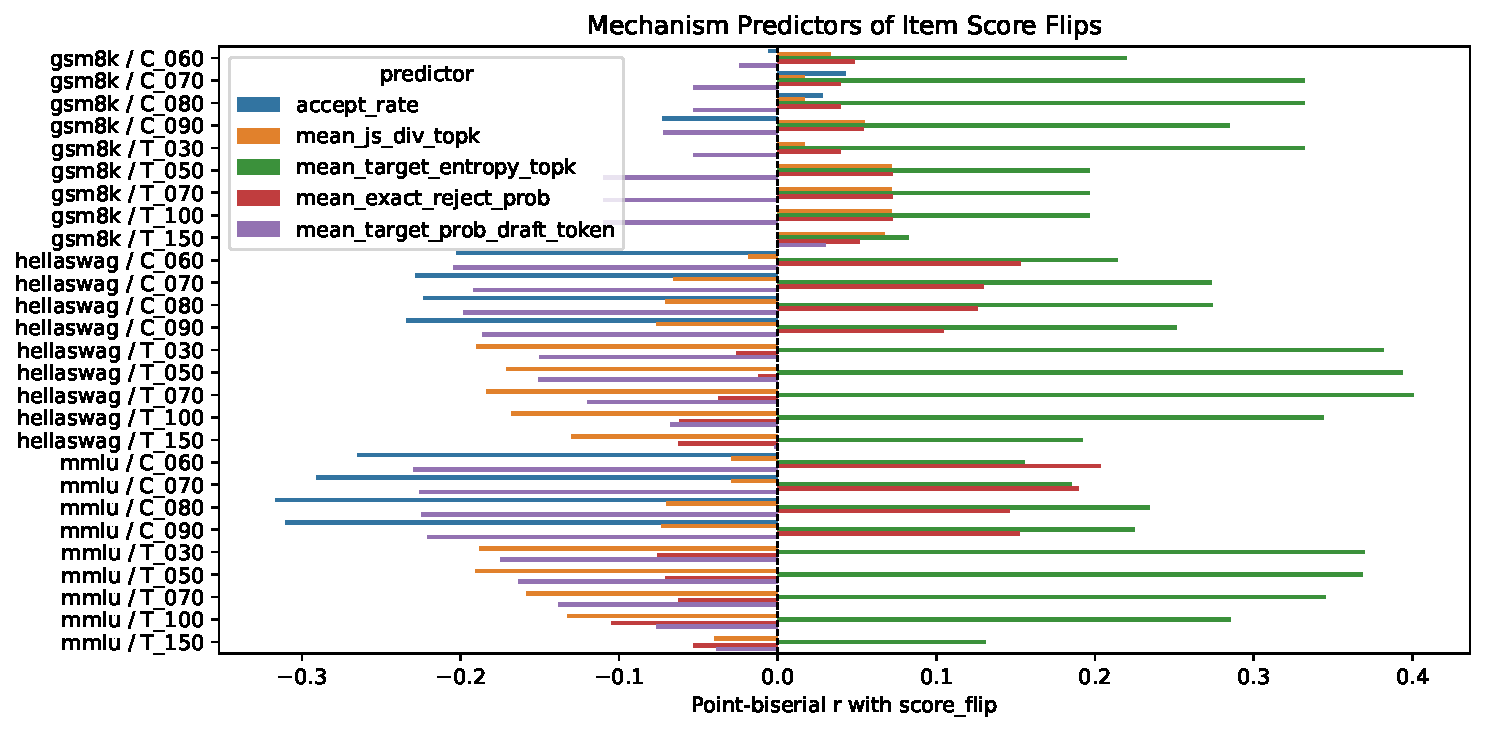
\includegraphics[width=0.92\linewidth]{results/fig_mechanism_flip_predictors.pdf}
\caption{Mechanism predictors of item score flips across benchmarks. Acceptance rate and target entropy are the strongest and most consistent predictors. Results are pooled across both model pairs for each benchmark. Associations are exploratory given the single-run design.}
\label{fig:mechanism}
\end{figure}

\subsection{Descriptive Variance Decomposition}

Table~\ref{tab:gtheory} reports the descriptive generalizability theory decomposition following \citet{cronbach1972dependability}. Because $N_{\text{RUNS}}{=}1$, run variance is excluded and the decomposition is treated as descriptive rather than inferential. Across all six benchmark--model combinations, item variance and item-by-condition interaction variance dominate, while condition variance is negligibly small.

\begin{table}[t]
\centering
\caption{Descriptive variance components from the $G$-study (run variance excluded; $N_{\text{RUNS}}{=}1$). Condition variance ($\hat\sigma^2_{\text{cond}}$) is consistently much smaller than item variance and item-by-condition interaction variance. The $G$ coefficient is computed as the proportion of variance explained by stable item-level signal.}
\label{tab:gtheory}
\small
\begin{tabular}{llrrrr}
\toprule
Model pair & Benchmark & $\hat\sigma^2_{\text{item}}$ & $\hat\sigma^2_{\text{cond}}$ & $\hat\sigma^2_{\text{item}\times\text{cond}}$ & $G$ \\
\midrule
Llama $\rightarrow$ Llama & GSM8K     & 0.0518 & 0.00231 & 0.0861 & $>$0.999 \\
Llama $\rightarrow$ Llama & HellaSwag & 0.1347 & 0.00486 & 0.2317 & $>$0.999 \\
Llama $\rightarrow$ Llama & MMLU      & 0.1444 & 0.00284 & 0.2438 & $>$0.999 \\
Qwen $\rightarrow$ Qwen   & GSM8K     & 0.1829 & 0.00063 & 0.1990 & $>$0.999 \\
Qwen $\rightarrow$ Qwen   & HellaSwag & 0.1285 & 0.00460 & 0.1758 & $>$0.999 \\
Qwen $\rightarrow$ Qwen   & MMLU      & 0.1405 & 0.00330 & 0.2212 & $>$0.999 \\
\bottomrule
\end{tabular}
\end{table}

The near-unity $G$ coefficients ($G > 0.999$ in all cases) reflect the fact that condition-level variance is trivially small relative to item variance---not that measurement is uniformly reliable. The large item-by-condition interaction terms ($\hat\sigma^2_{\text{item}\times\text{cond}} \approx 0.09$--$0.24$) indicate that individual items respond differentially to decoding perturbations even when aggregate scores are stable, consistent with the item-flip analysis. This decomposition supports the view that decoding condition is a relatively small but non-zero measurement facet whose influence is item-specific rather than uniformly distributed.

\begin{figure}[t]
\centering
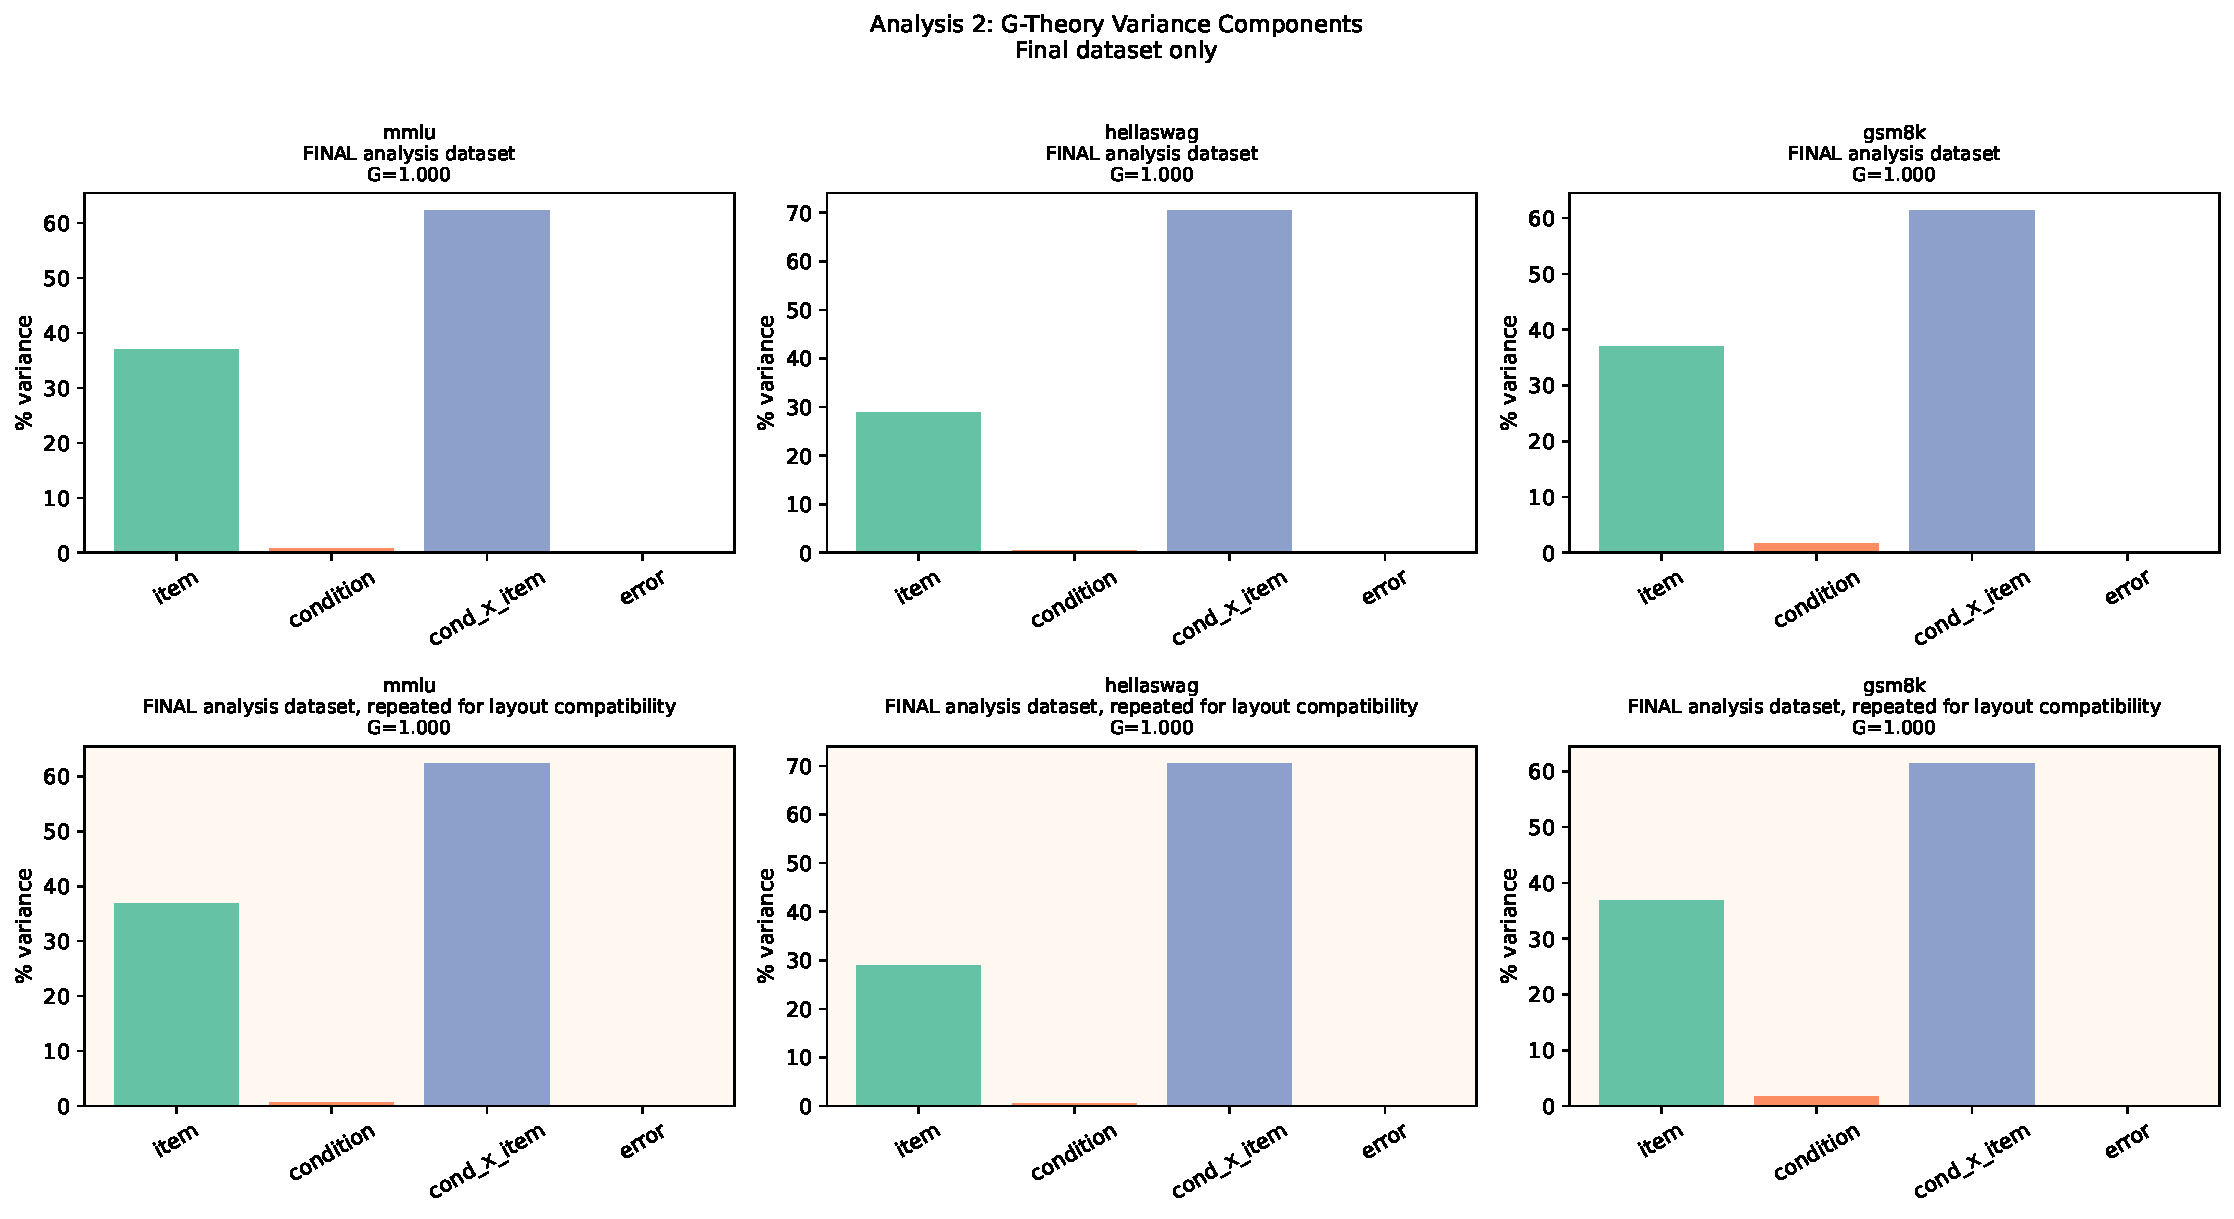
\includegraphics[width=0.95\linewidth]{results/fig2_gtheory_comparison.pdf}
\caption{Descriptive variance decomposition over items and decoding conditions. Condition variance is negligible in absolute terms, but item-by-condition interaction variance is substantial, reflecting heterogeneous item sensitivity to the decoding perturbation.}
\label{fig:gtheory}
\end{figure}

\section{Discussion}

\paragraph{Exact speculation is measurement-invariant.} The null result for exact speculative decoding (Condition $B$) is the most important positive finding. In Messick's validity framework~\citep{messick1995validity}, a measurement procedure is construct-valid to the extent that observed scores reflect the intended capability without contamination from irrelevant sources. Exact speculation, by construction, should recover the target distribution; this analysis confirms empirically that it does so at the item level across 2,400 paired item evaluations. Benchmark practitioners who need exact distributional fidelity have a verified option.

\paragraph{Approximate speculation is a moderate measurement facet.} Approximate speculation introduced statistically significant score-level changes in only one benchmark--model combination (Llama GSM8K at $\alpha \leq 0.80$, Bonferroni-corrected $p = 0.00092$). On MMLU and HellaSwag, score-level changes did not reach significance for either model pair. However, the large item-by-condition interaction variance in the $G$-study indicates that individual items are differentially sensitive to the decoding perturbation even when aggregate scores appear stable. This distinction matters for measurement validity: construct-irrelevant variance~\citep{messick1995validity} can manifest at the item level without surfacing at the score level.

\paragraph{Token perturbation does not imply score perturbation.} Token-change rates reached 100\% on GSM8K, 13\%--25\% on HellaSwag, and 16\%--23\% on MMLU under approximate speculation, yet score flip rates were usually smaller (e.g., silent-change fraction up to 0.96 for Qwen GSM8K at $C_{.60}$). Score-level analysis alone is therefore insufficient to detect inference-induced response-process variation.

\paragraph{Temperature establishes a practical reference scale.} Temperature perturbations produced larger and more statistically robust score shifts than approximate speculation on every benchmark, with especially strong monotone effects on MMLU and HellaSwag ($r \approx -0.97$ to $-1.00$). This validates the measurement framework and contextualizes the practical significance of speculation effects: in most combinations studied, approximate speculation induces changes smaller than the largest temperature perturbations.

\paragraph{Mechanism: uncertainty amplifies susceptibility.} The mechanism analysis identifies target-distribution entropy and acceptance rate as the primary predictors of item-level score flips. Items where the target model is uncertain (high entropy) and the draft model's token diverges from the target (low acceptance rate) are most susceptible to score changes under approximate speculation. This is theoretically coherent: approximate speculation effectively substitutes draft tokens for target tokens at a rate determined by the acceptance threshold, and this substitution is most likely to alter item outcomes when the target model's preference is weakly expressed. From a measurement-science perspective, this identifies a principled approach to \emph{inference-sensitive item detection}: high-entropy items under a given draft--target pair are at elevated risk of score perturbation if approximate speculation is used.

\section{Limitations}

\paragraph{Single run.} The analysis uses $N_{\text{RUNS}}{=}1$. All inference is over items, not over repeated stochastic generations. Run-to-run reliability cannot be estimated from this data, and regression slopes from the mechanism analysis should be treated as descriptive. A fully crossed $G$-study with item, run, and condition facets would require at least $R = 5$ independent runs per condition.

\paragraph{IRT and DIF analysis not feasible.} The pre-analysis plan specified a 2PL IRT model with differential item functioning (DIF) analysis. With only two evaluated model instances, IRT estimation is not identifiable; a meaningful DIF analysis requires $N_{\text{models}} \geq 10$--$20$ per condition.

\paragraph{Benchmark and model scope.} The analysis covers only Qwen2.5 and Llama 3.x families and three benchmark formats. HellaSwag and MMLU use 500-item subsets, while GSM8K uses 200 projected items, so generalizability to other model families, longer generations, and full benchmark distributions remains unknown.

\paragraph{Logit-replay approximation.} The logit-replay design enables exact paired comparisons but approximates true autoregressive generation, particularly for multi-step GSM8K sequences. Full autoregressive evaluation would be more realistic but substantially more expensive.

\section{Conclusion}

This project evaluates speculative decoding as a potential source of construct-irrelevant measurement variance in LLM benchmarking, using a paired item-level design across three benchmark constructs and two model families. The main findings are:

\begin{enumerate}
    \item \textbf{Exact speculation is measurement-preserving.} $b=c=0$, $p=1.0$ across all benchmark--model combinations, empirically validating the theoretical guarantee at the item level.
    \item \textbf{Approximate speculation can shift scores significantly.} The largest Bonferroni-significant effect was $-8.5$ pp on Llama GSM8K at $\alpha \leq 0.80$ ($p_{\text{Bonferroni}} = 0.00092$); MMLU and HellaSwag effects did not reach significance.
    \item \textbf{Token perturbation substantially exceeds score perturbation.} Score-level analysis alone can miss inference-induced response-process variation.
    \item \textbf{Temperature is a stronger reference perturbation.} MMLU and HellaSwag Pearson correlations are strongly negative ($r \approx -0.97$ to $-1.00$, $p < 0.01$); speculative decoding effects are generally smaller than the largest temperature perturbations.
    \item \textbf{High-entropy items are most susceptible.} Target entropy predicts score flips ($r_{\text{pb}} = 0.185$--$0.332$), providing a principled criterion for identifying inference-sensitive items.
\end{enumerate}

Benchmark practitioners using speculative decoding should report whether exact or approximate variants were used and at what threshold. Exact speculation is safe; aggressive approximate speculation ($\alpha \leq 0.80$) can introduce score-level effects that are smaller than temperature perturbations but still large enough to matter for benchmark interpretation. Future work should add multiple stochastic runs, expand to more model families to enable IRT-based DIF analysis, and conduct a fully crossed $G$-study with item, model, condition, and run facets.

\section*{Reproducibility Statement}

All analyses are computed from logits collected on an NVIDIA L4 GPU and saved result files. MMLU and HellaSwag use 500 observed items each; GSM8K uses 200 projected item evaluations. The notebook fixes random seeds and writes all figures and tables to the \texttt{results/} directory. Reproducing the full data collection requires re-generating the logits on compatible hardware; reproducing all reported analyses and figures uses the saved logits and result files provided with the submission.

\begin{thebibliography}{99}

\bibitem[Leviathan et al.(2023)]{leviathan2023fast}
Yaniv Leviathan, Matan Kalman, and Yossi Matias.
\newblock Fast inference from transformers via speculative decoding.
\newblock In \emph{International Conference on Machine Learning}, 2023.

\bibitem[Chen et al.(2023)]{chen2023accelerating}
Charlie Chen, Sebastian Borgeaud, Geoffrey Irving, Jean-Baptiste Lespiau, Laurent Sifre, and John Jumper.
\newblock Accelerating large language model decoding with speculative sampling.
\newblock \emph{arXiv preprint arXiv:2302.01318}, 2023.

\bibitem[Miao et al.(2024)]{miao2024specinfer}
Xupeng Miao, Gabriele Oliaro, Zhihao Zhang, Xinhao Cheng, Zeyu Wang, Rae Ying Yee Wong, Zhuoming Chen, Daiyaan Arfeen, Reyna Abhyankar, and Zhihao Jia.
\newblock SpecInfer: Accelerating large language model serving with tree-based speculative inference and verification.
\newblock In \emph{Proceedings of the 29th ACM International Conference on Architectural Support for Programming Languages and Operating Systems}, 2024.

\bibitem[Hendrycks et al.(2021)]{hendrycks2021mmlu}
Dan Hendrycks, Collin Burns, Steven Basart, Andy Zou, Mantas Mazeika, Dawn Song, and Jacob Steinhardt.
\newblock Measuring massive multitask language understanding.
\newblock In \emph{International Conference on Learning Representations}, 2021.

\bibitem[Zellers et al.(2019)]{zellers2019hellaswag}
Rowan Zellers, Ari Holtzman, Yonatan Bisk, Ali Farhadi, and Yejin Choi.
\newblock HellaSwag: Can a machine really finish your sentence?
\newblock In \emph{Annual Meeting of the Association for Computational Linguistics}, 2019.

\bibitem[Cobbe et al.(2021)]{cobbe2021gsm8k}
Karl Cobbe, Vineet Kosaraju, Mohammad Bavarian, Mark Chen, Heewoo Jun, Lukasz Kaiser, Matthias Plappert, Jerry Tworek, Jacob Hilton, Reiichiro Nakano, Christopher Hesse, and John Schulman.
\newblock Training verifiers to solve math word problems.
\newblock \emph{arXiv preprint arXiv:2110.14168}, 2021.

\bibitem[Cronbach et al.(1972)]{cronbach1972dependability}
Lee J. Cronbach, Goldine C. Gleser, Harinder Nanda, and Nageswari Rajaratnam.
\newblock \emph{The Dependability of Behavioral Measurements: Theory of Generalizability for Scores and Profiles}.
\newblock Wiley, 1972.

\bibitem[Messick(1995)]{messick1995validity}
Samuel Messick.
\newblock Validity of psychological assessment: Validation of inferences from persons' responses and performances as scientific inquiry into score meaning.
\newblock \emph{American Psychologist}, 50(9):741--749, 1995.

\bibitem[Ribeiro et al.(2020)]{ribeiro2020beyond}
Marco Tulio Ribeiro, Tongshuang Wu, Carlos Guestrin, and Sameer Singh.
\newblock Beyond accuracy: Behavioral testing of NLP models with CheckList.
\newblock In \emph{Annual Meeting of the Association for Computational Linguistics}, 2020.

\bibitem[Gururangan et al.(2018)]{gururangan2018annotation}
Suchin Gururangan, Swabha Swayamdipta, Omer Levy, Roy Schwartz, Samuel Bowman, and Noah A. Smith.
\newblock Annotation artifacts in natural language inference data.
\newblock In \emph{North American Chapter of the Association for Computational Linguistics}, 2018.

\bibitem[Ethayarajh \& Jurafsky(2022)]{ethayarajh2022authenticity}
Kawin Ethayarajh and Dan Jurafsky.
\newblock Authenticity of machine learning in an age of unreliable baselines.
\newblock \emph{Transactions of the Association for Computational Linguistics}, 10:437--454, 2022.

\bibitem[Dodge et al.(2020)]{dodge2020fine}
Jesse Dodge, Gabriel Ilharco, Roy Schwartz, Ali Farhadi, Hannaneh Hajishirzi, and Noah Smith.
\newblock Fine-tuning pretrained language models: Weight initializations, data orders, and early stopping.
\newblock \emph{arXiv preprint arXiv:2002.06305}, 2020.

\bibitem[Bouthillier et al.(2021)]{bouthillier2021accounting}
Xavier Bouthillier, Pierre Delaunay, Mirko Bronzi, Amy Trofimov, Brennan Nichyporuk, Justin Szeto, Naz Sepah, Edward Raff, Kanika Madan, Vikram Voleti, Samira Ebrahimi Kahou, Vincent Michalski, Dmitriy Serdyuk, Tal Arbel, Chris Pal, Gaël Varoquaux, and Pascal Vincent.
\newblock Accounting for variance in machine learning benchmarks.
\newblock In \emph{Proceedings of Machine Learning and Systems}, 2021.

\bibitem[Liang et al.(2022)]{liang2022holistic}
Percy Liang, Rishi Bommasani, Tony Lee, et al.
\newblock Holistic evaluation of language models.
\newblock \emph{Transactions on Machine Learning Research}, 2022.

\end{thebibliography}

\appendix

\section{Additional Figures}

\begin{figure}[h]
\centering
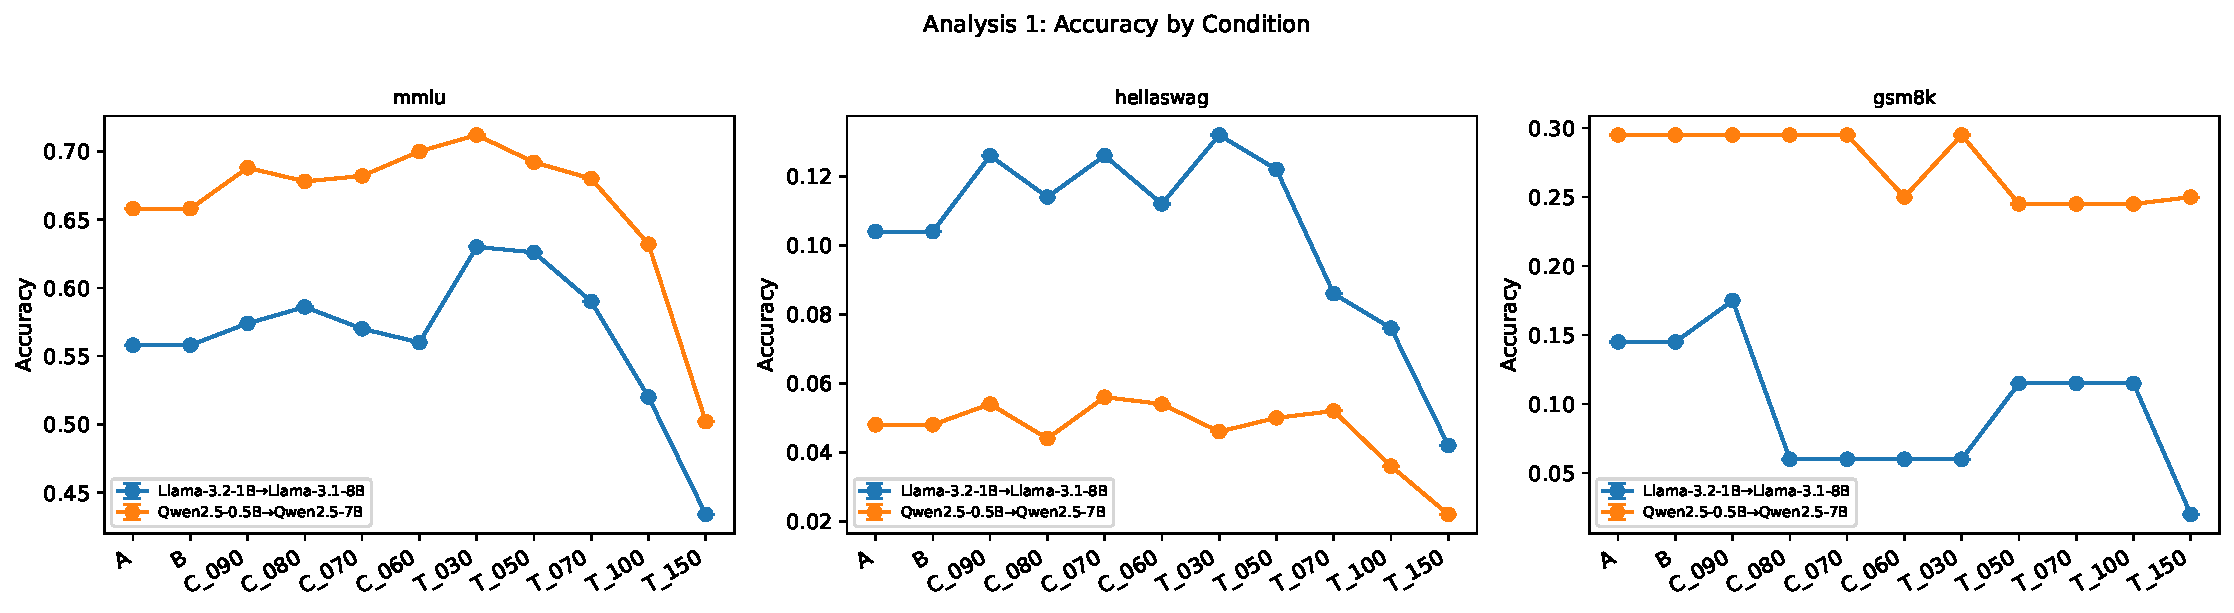
\includegraphics[width=0.95\linewidth]{results/fig1_accuracy_comparison.pdf}
\caption{Accuracy by decoding condition for all benchmark--model combinations (left to right: Baseline, Exact, Approximate, Temperature).}
\end{figure}

\begin{figure}[h]
\centering
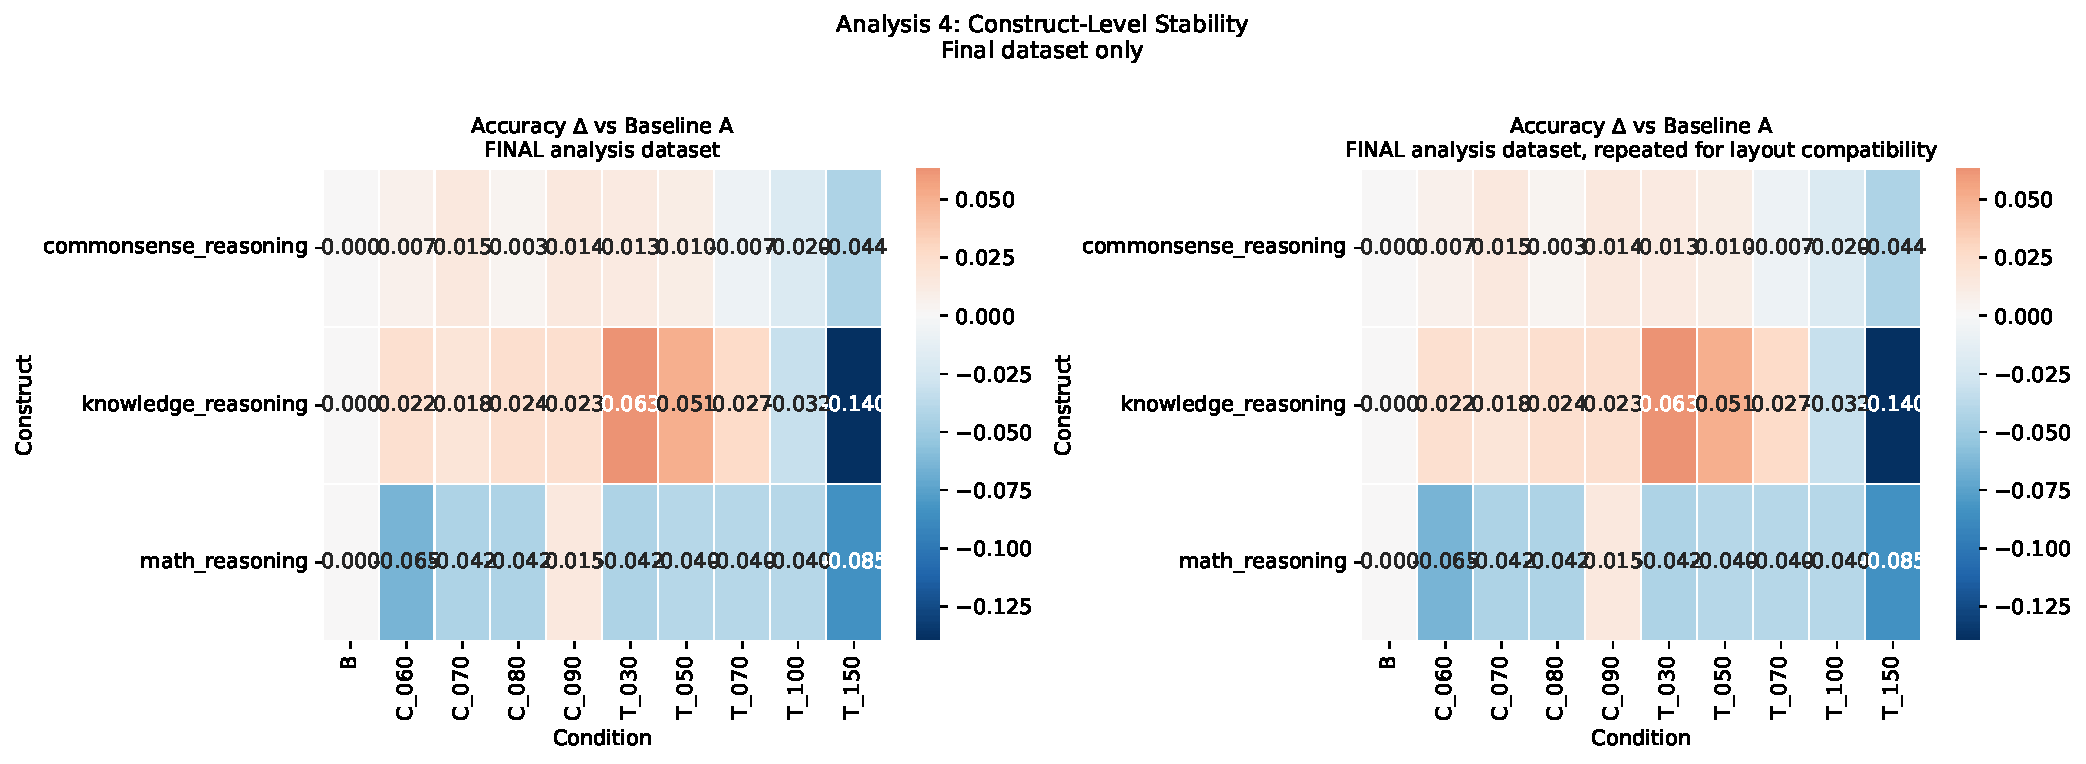
\includegraphics[width=0.95\linewidth]{results/fig4_construct_comparison.pdf}
\caption{Construct-level accuracy changes relative to baseline. Temperature effects are larger and more monotone than speculative decoding effects.}
\end{figure}

\begin{figure}[h]
\centering
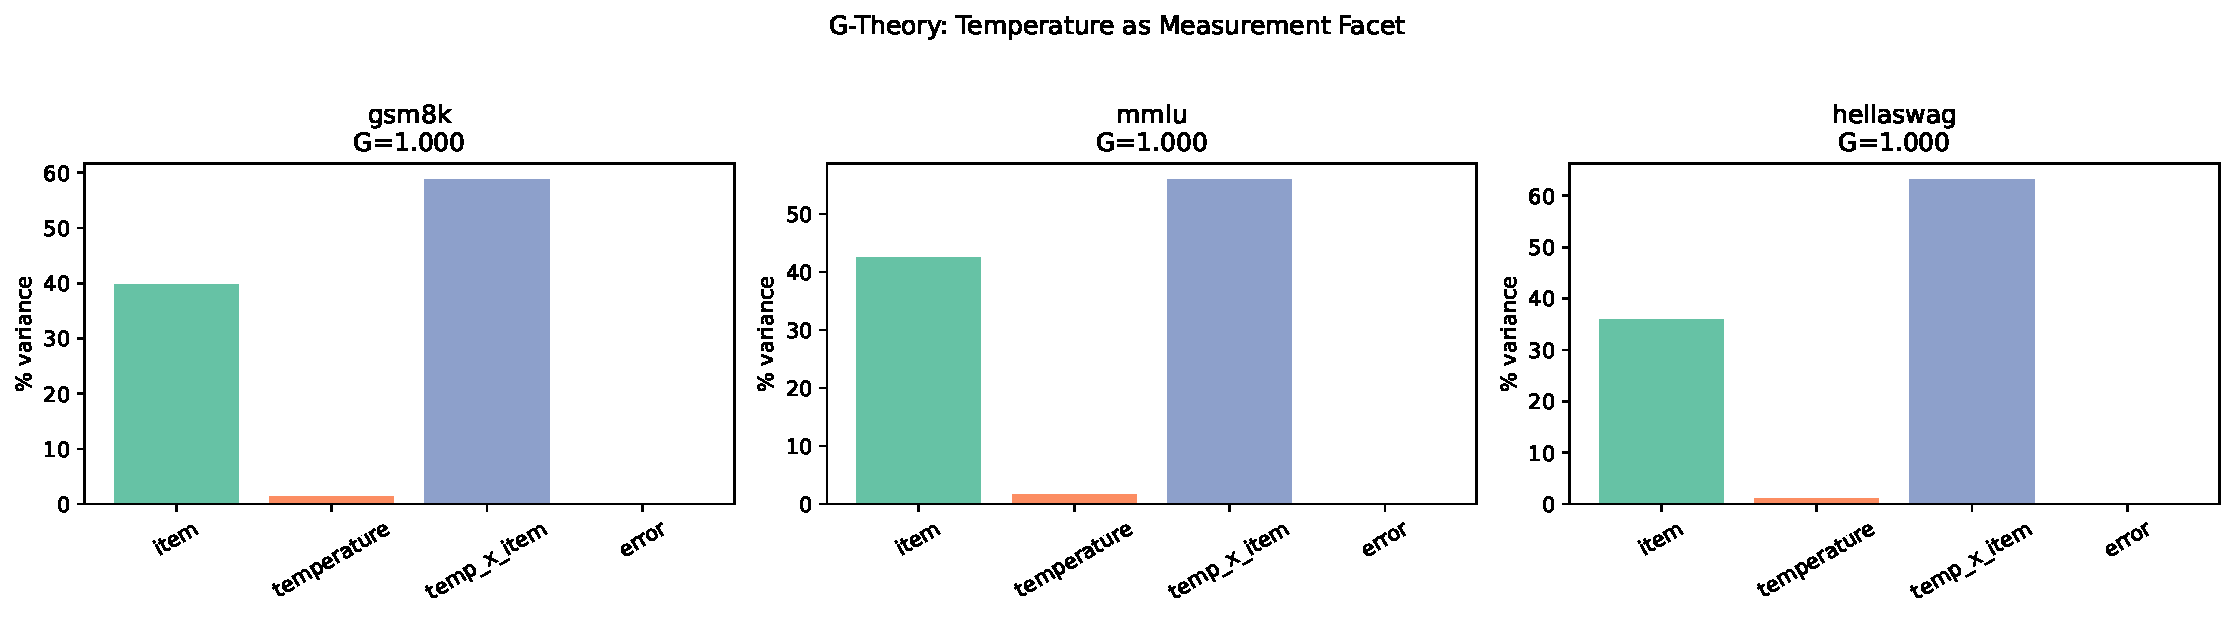
\includegraphics[width=0.85\linewidth]{results/fig_temp_gtheory.pdf}
\caption{Descriptive temperature-facet variance decomposition. Variance contributions mirror the speculative decoding decomposition in Table~\ref{tab:gtheory}.}
\end{figure}

\end{document}
